\chapter{Divide and Conquer, Recurrences, and the Master Theorem}

There is a single idea hiding inside an astonishing number of fast algorithms.
You have probably already used it without naming it. Suppose a friend hands you a
thick phone book and asks you to find the listing for ``Okonkwo.'' You do not
start at page one and read every name. You flip to the middle, see that you have
landed on the ``M'' pages, and instantly throw away the entire first half of the
book. You repeat. Each glance discards half of what remains. A book of a million
names is conquered in about twenty glances.

That move --- \emph{cut the problem into smaller copies of itself, solve those,
and stitch the answers back together} --- is the whole subject of this chapter.
We will slow it down until it is almost embarrassing, then build it back
up into one of the sharpest design techniques you own. Along the way we have
to learn how to \emph{count} the work such algorithms do, which leads to
\emph{recurrences} and to a remarkable shortcut for solving them called the
\emph{master theorem}.

\begin{focusbox}
By the end of this chapter you should be able to: (1) recognize when a problem
splits into independent subproblems; (2) write down a recurrence $T(n)$ that
describes the running time of a recursive algorithm; (3) solve that recurrence
three different ways --- by guessing and proving (substitution), by drawing a
recursion tree, and by plugging into the master theorem; and (4) read the answer
the master theorem gives and \emph{feel} why it is true.
\end{focusbox}

\begin{historybox}
In the autumn of 1960 at Moscow State University, the towering mathematician Andrei Kolmogorov
convened a seminar on cybernetics and put forward his famous $n^2$ conjecture: that multiplying two
$n$-digit numbers inherently demands $\Omega(n^2)$ bit operations. For millennia, grade-school
multiplication had reigned unchallenged; it seemed self-evident that every digit of one number must
touch every digit of the other. Sitting in the audience was a 23-year-old student named Anatoly
Karatsuba. Within a single week, Karatsuba noticed a magical algebraic identity: by expanding
$(x_1 B + x_0)(y_1 B + y_0)$ with a clever cross-term grouping, he could replace four half-sized
multiplications with just three! That one saved multiplication shifted the recurrence to
$T(n) = 3T(n/2) + O(n)$, shattering the quadratic wall down to
$\Theta(n^{\log_2 3}) \approx \Theta(n^{1.585})$. Stunned, Kolmogorov immediately terminated the
seminar, wrote up the breakthrough paper himself, and submitted it for publication. Nine years later,
in 1969, Volker Strassen delivered an even greater shock to numerical linear algebra by showing that
$2 \times 2$ matrices could be multiplied with $7$ multiplications instead of $8$, collapsing the
centuries-old $\Theta(n^3)$ matrix barrier to $\Theta(n^{2.807})$.

The central lesson of divide-and-conquer is that simply splitting a problem into smaller pieces is
not enough. If you chop an $n \times n$ matrix into eight half-sized blocks, the recurrence
$T(n) = 8T(n/2) + \Theta(n^2)$ still yields $\Theta(n^3)$ --- the branching factor $a=8$
overwhelms the division, yielding zero asymptotic speedup. The breakthrough only happens when you
mathematically reduce the branching factor. In 1980, Jon Bentley, Dorothea Haken, and James B. Saxe
unified these recurrence solutions into the \emph{Master Theorem}, turning what once required
page-long induction proofs into a three-case comparison between the recursive branching
$n^{\log_b a}$ and the work $f(n)$ done at each step.

Divide-and-conquer unlocked sub-quadratic multiplication, sub-cubic matrix algebra, and optimal
$\Theta(n \log n)$ comparison sorting. But its algebraic triumph carries honest practical burdens:
large constant factors and recursive overhead. Strassen's algorithm requires eighteen matrix
additions per step, making it slower than standard multiplication until matrices reach dimensions
past a thousand. Furthermore, when subproblems overlap rather than dividing cleanly --- as in
recursive Fibonacci calculations --- divide-and-conquer fails catastrophically, blowing up into
exponential $\Theta(2^n)$ repetition. In Chapter~15, we introduce Dynamic Programming to solve the
dilemma of overlapping subproblems, and in Chapter~29 we push divide-and-conquer to its theoretical
summit with the Fast Fourier Transform, multiplying polynomials in $\Theta(n \log n)$ time.
\end{historybox}

\section{The shape of a divide-and-conquer algorithm}

Every divide-and-conquer algorithm has the same three-beat rhythm. Memorize the
rhythm and most of these algorithms will feel like variations on one tune.

\begin{intuitionbox}
\textbf{Divide.} Break the problem into a few smaller subproblems that are
\emph{the same kind of problem}, just smaller.

\textbf{Conquer.} Solve each subproblem \emph{recursively} --- call the very same
procedure on the smaller input. Once the subproblem is tiny enough (often size
$1$), solve it directly; that tiny case is the \emph{base case}.

\textbf{Combine.} Glue the subproblem answers together into an answer for the
original problem.
\end{intuitionbox}

The word ``recursively'' in the conquer step carries most of the weight. We do not
write three separate algorithms for the three sizes of the problem; we write
\emph{one} algorithm that calls itself. Each call shrinks the input, and because
inputs cannot shrink forever, the chain of calls must eventually bottom out at the
base case. That is the same logic as a proof by induction, and for good reason:
correctness of a divide-and-conquer algorithm is almost always an induction
proof in disguise.

\begin{focusbox}
The two questions you must answer for \emph{any} divide-and-conquer design:
(1) \emph{What is the base case, and why is its solution directly verifiable?}
(2) \emph{If the recursive calls return correct answers on the smaller inputs,
does the combine step produce a correct answer on the whole input?}
If both are ``yes,'' induction guarantees the algorithm is correct on every size.
\end{focusbox}

\subsection{A first, familiar example: binary search}

Here is the phone-book story written as code. Binary search looks for a value
$x$ in a \emph{sorted} array $A[1\ldots n]$.

\begin{algorithm}[H]
\caption{\textsc{Binary-Search}$(A, x, lo, hi)$}
\KwIn{A sorted array $A$, a target $x$, and bounds $lo \le hi+1$.}
\KwOut{An index $i$ with $A[i]=x$, or \textsc{Nil} if $x$ is absent.}
\If{$lo > hi$}{\Return \textsc{Nil}\tcp*{base case: empty range}}
$mid \gets \floor{(lo+hi)/2}$\;
\If{$A[mid] = x$}{\Return $mid$}
\ElseIf{$A[mid] > x$}{\Return \textsc{Binary-Search}$(A, x, lo, mid-1)$\tcp*{left half}}
\Else{\Return \textsc{Binary-Search}$(A, x, mid+1, hi)$\tcp*{right half}}
\end{algorithm}

Divide: compare against the middle and pick a half. Conquer: search that half
recursively. Combine: nothing to do --- the half's answer \emph{is} our answer.
This is the friendliest kind of divide-and-conquer, where ``divide'' throws away
work for free and ``combine'' is trivial. How long does it take? Each call does a
constant amount of work (one comparison, some arithmetic) and then makes one call
on a problem of half the size. If $T(n)$ is the time on a range of $n$ elements,
$$T(n) = T(n/2) + c.$$
We will learn to read that line like a sentence. For now, trust the phone-book
count: about $\log_2 n$ halvings, each costing $c$, so $T(n) = \Th(\log n)$.

\section{Merge sort, revisited slowly}

You may have met merge sort already. We meet it again here, more
carefully, because it is the cleanest possible illustration of the paradigm and
because its analysis sets up everything else.

\subsection{The idea}

\begin{intuitionbox}
To sort a pile of $n$ cards: if the pile is a single card, it is already sorted ---
done. Otherwise split the pile into two halves, sort each half (by the same
method, recursively), and then \emph{merge} the two sorted halves into one sorted
pile. Merging is easy because both halves are already sorted: repeatedly take the
smaller of the two top cards.
\end{intuitionbox}

The clever part is \emph{merge}, the combine step. Given two sorted lists, you can
zip them together into one sorted list in a single pass. Keep a finger on the
front of each list; compare the two fingered elements; copy the smaller one out
and advance that finger. When one list empties, copy the rest of the other.
Figure~\ref{ch04:mergefig} shows a single merge step frozen mid-zip.

\begin{figure}[H]
\centering
\begin{tikzpicture}[font=\small,>=Stealth,
  cell/.style={draw,minimum width=7mm,minimum height=7mm,inner sep=0pt}]
% L row
\node at (-1.4,0) {$L$:};
\foreach \v/\x [count=\i from 0] in {2/0,4/1,5/2,7/3}{
  \node[cell] (L\i) at (\x*0.8,0) {\v};
}
% R row
\node at (-1.4,-1.2) {$R$:};
\foreach \v/\x [count=\i from 0] in {1/0,2/1,3/2,6/3}{
  \node[cell] (R\i) at (\x*0.8,-1.2) {\v};
}
% fingers: suppose L finger at index 1 (value 4), R finger at index 2 (value 3)
\draw[->,sourceblue,thick] (L1.north)+(0,0.5) -- (L1.north);
\node[sourceblue] at ($(L1.north)+(0,0.75)$) {\tiny $i$};
\draw[->,targetgreen,thick] ($(R2.south)+(0,-0.5)$) -- (R2.south);
\node[targetgreen] at ($(R2.south)+(0,-0.72)$) {\tiny $j$};
% output row
\node at (-1.4,-2.7) {out:};
\foreach \v/\x [count=\i from 0] in {1/0,2/1,2/2,3/3}{
  \node[cell,fill=gray!12] (O\i) at (\x*0.8,-2.7) {\v};
}
\foreach \x in {4,5,6,7}{
  \node[cell] at (\x*0.8,-2.7) {};
}
\node[align=left] at (5.6,-1.0)
  {\footnotesize compare $L[i]{=}4$\\[-2pt]\footnotesize vs $R[j]{=}3$:\\[-2pt]
   \footnotesize emit $3$, advance $j$};
\end{tikzpicture}
\caption{One step of \textsc{Merge}. Two fingers $i,j$ scan the sorted inputs
$L$ and $R$; the smaller fingered value is copied to the output and its finger
advances. Here $4>3$, so $3$ is emitted and $j$ steps right.}
\label{ch04:mergefig}
\end{figure}

\begin{algorithm}[H]
\caption{\textsc{Merge}$(A, lo, mid, hi)$}
\KwIn{$A[lo\ldots mid]$ and $A[mid+1\ldots hi]$ are each sorted.}
\KwOut{$A[lo\ldots hi]$ sorted, in place.}
$L \gets A[lo\ldots mid]$ with a $+\infty$ sentinel appended\;
$R \gets A[mid+1\ldots hi]$ with a $+\infty$ sentinel appended\;
$i \gets 1$; \quad $j \gets 1$\;
\For{$k \gets lo$ \KwTo $hi$}{
  \If{$L[i] \le R[j]$}{$A[k] \gets L[i]$; \quad $i \gets i+1$}
  \Else{$A[k] \gets R[j]$; \quad $j \gets j+1$}
}
\end{algorithm}

The $+\infty$ sentinels are a small trick so we never have to check ``has this
list run out?'' inside the loop: once a real list is exhausted, its finger sits on
$+\infty$, which loses every comparison, so the other list drains naturally.

\begin{algorithm}[H]
\caption{\textsc{Merge-Sort}$(A, lo, hi)$}
\KwIn{An array $A$ and bounds $lo \le hi$.}
\KwOut{$A[lo\ldots hi]$ sorted in nondecreasing order.}
\If{$lo \ge hi$}{\Return\tcp*{base case: 0 or 1 element, already sorted}}
$mid \gets \floor{(lo+hi)/2}$\;
\textsc{Merge-Sort}$(A, lo, mid)$\tcp*{conquer left}
\textsc{Merge-Sort}$(A, mid+1, hi)$\tcp*{conquer right}
\textsc{Merge}$(A, lo, mid, hi)$\tcp*{combine}
\end{algorithm}

\subsection{A full numeric trace}

Let us sort $A = [5,\,2,\,4,\,7,\,1,\,3,\,2,\,6]$ ($n=8$). I will draw the
recursion as a tree: splitting on the way down, merging on the way up.

\begin{labbox}
\textbf{Trace it yourself.} Cover the answers below and run the splits in your
head before peeking.

\textbf{Splitting down:}
\begin{itemize}
\item $[5,2,4,7,1,3,2,6] \to [5,2,4,7]$ and $[1,3,2,6]$
\item $[5,2,4,7] \to [5,2]$ and $[4,7]$; \quad $[1,3,2,6] \to [1,3]$ and $[2,6]$
\item $[5,2] \to [5],[2]$; \; $[4,7]\to[4],[7]$; \; $[1,3]\to[1],[3]$; \;
      $[2,6]\to[2],[6]$
\end{itemize}

\textbf{Merging up:}
\begin{itemize}
\item $[5],[2] \to [2,5]$; \; $[4],[7]\to[4,7]$; \; $[1],[3]\to[1,3]$; \;
      $[2],[6]\to[2,6]$
\item $[2,5],[4,7] \to [2,4,5,7]$; \quad $[1,3],[2,6]\to[1,2,3,6]$
\item $[2,4,5,7],[1,2,3,6] \to [1,2,2,3,4,5,6,7]$
\end{itemize}
\end{labbox}

Watch the last merge in slow motion. Fingers start at the fronts of
$L=[2,4,5,7]$ and $R=[1,2,3,6]$.

\begin{center}
\begin{tabular}{cllll}
\toprule
step & compare & emit & $L$ remaining & $R$ remaining \\
\midrule
1 & $2$ vs $1$ & $1$ & $2,4,5,7$ & $2,3,6$ \\
2 & $2$ vs $2$ & $2$ & $4,5,7$   & $2,3,6$ \\
3 & $4$ vs $2$ & $2$ & $4,5,7$   & $3,6$ \\
4 & $4$ vs $3$ & $3$ & $4,5,7$   & $6$ \\
5 & $4$ vs $6$ & $4$ & $5,7$     & $6$ \\
6 & $5$ vs $6$ & $5$ & $7$       & $6$ \\
7 & $7$ vs $6$ & $6$ & $7$       & --- \\
8 & ($R$ empty) & $7$ & ---       & --- \\
\bottomrule
\end{tabular}
\end{center}

Output: $[1,2,2,3,4,5,6,7]$. Notice step 2: when the two fingered elements tie, we
took from $L$ because the test is $L[i] \le R[j]$. That choice makes merge sort
\emph{stable} (equal elements keep their original relative order), a property
that matters more than you would guess in real systems.

\begin{trapbox}
The merge step needs \emph{extra space} for the copies $L$ and $R$ --- merge sort
is not in place. A classic mistake is to assume you can merge two halves of one
array back into that same array without a scratch buffer. You cannot do it in
$O(1)$ extra space without a much fancier algorithm; the straightforward merge
uses $\Th(n)$ auxiliary memory. (We will revisit this trade-off in the cost
summary.)
\end{trapbox}

\subsection{Why it is correct}

\begin{formalbox}
\textbf{Claim.} \textsc{Merge-Sort}$(A, lo, hi)$ leaves $A[lo\ldots hi]$ sorted.

\textbf{Proof by strong induction on $m = hi - lo + 1$, the number of elements.}

\emph{Base case} ($m \le 1$): a range of $0$ or $1$ element is sorted by
definition, and the algorithm returns without touching it. True.

\emph{Inductive step} ($m \ge 2$): assume the claim holds for all ranges of fewer
than $m$ elements. Since $m \ge 2$, the two recursive calls operate on ranges of
sizes $\ceil{m/2}$ and $\floor{m/2}$, both strictly less than $m$ and both at
least $1$. By the inductive hypothesis, after the two calls $A[lo\ldots mid]$ and
$A[mid+1\ldots hi]$ are each sorted. \textsc{Merge} then combines two sorted
ranges into one sorted range (this is the merge \emph{lemma}; prove it as a loop
invariant: ``at the start of iteration $k$, $A[lo\ldots k-1]$ holds the $k-lo$
smallest of the merged elements, in order, and $L[i], R[j]$ are the smallest
not-yet-copied elements of each list''). Hence $A[lo\ldots hi]$ is sorted.
By induction the claim holds for all $m$. $\qquad\blacksquare$
\end{formalbox}

That is the entire shape of a divide-and-conquer correctness proof, and you will
reuse it constantly: base case obvious, recursive calls correct by hypothesis,
combine step correct by a small lemma.

\section{Counting the work: recurrences}

Now the analysis. How long does \textsc{Merge-Sort} take on $n$ elements? The
answer is itself recursive, because the algorithm is recursive. Let $T(n)$
denote the worst-case running time on an input of size $n$. Reading the code:

\begin{itemize}
\item If $n \le 1$, we do a constant amount of work: $T(n) = \Th(1)$.
\item If $n > 1$, we make two recursive calls, each on half the input, costing
      $T(n/2)$ each. Computing $mid$ is constant. \textsc{Merge} on $n$ elements
      runs a single loop of $n$ iterations, so it costs $\Th(n)$.
\end{itemize}

Putting those together gives the \emph{recurrence}
$$
T(n) =
\begin{cases}
\Th(1) & \text{if } n \le 1,\\[2pt]
2\,T(n/2) + \Th(n) & \text{if } n > 1.
\end{cases}
$$

\begin{definition}[Recurrence]
A \emph{recurrence} is an equation that defines a function (here, the running time
$T$) in terms of its own values on smaller inputs, together with one or more base
cases. Solving a recurrence means finding a closed-form bound --- usually a
$\Th(\cdot)$ bound --- that does not refer to $T$ on the right-hand side.
\end{definition}

\begin{focusbox}
Two conventions we will lean on throughout, because they never change the
asymptotic answer for the algorithms in this book.
\textbf{(1) Floors and ceilings.} We write $T(n/2)$ even though the true sizes are
$\ceil{n/2}$ and $\floor{n/2}$. \textbf{(2) Small base cases.} We treat
$T(n)=\Th(1)$ for $n$ below some constant. Both simplifications are justified
rigorously in CLRS; we lean on them so the algebra stays clean.
\end{focusbox}

Three tools solve recurrences, and we will learn all three, because
each teaches you something the others hide.

\section{Method 1: the recursion tree (see the work)}

The recursion tree turns a recurrence into a picture you can literally add up.
Draw a node for the top-level call and label it with the \emph{non-recursive}
work that call does --- for merge sort, that is the $cn$ cost of merging, not the
recursive calls. Then draw its children: the subproblems it spawns. Repeat until
you hit base cases. Finally, sum the labels.

\subsection{Merge sort's tree}

For $T(n) = 2T(n/2) + cn$, the root does $cn$ work and has two children of size
$n/2$. Each of those does $c(n/2)$ work and has two children of size $n/4$, and so
on.

\begin{center}
\begin{tikzpicture}[
    level distance=12mm,
    level 1/.style={sibling distance=48mm},
    level 2/.style={sibling distance=24mm},
    every node/.style={font=\small},
    pnode/.style={draw,rounded corners,fill=sourceblue!10,inner sep=3pt},
    ann/.style={font=\footnotesize,gray!80!black}
  ]
\node[pnode] (root) {$cn$}
  child {node[pnode] {$c\,\tfrac{n}{2}$}
    child {node[pnode] {$c\,\tfrac{n}{4}$}
      child {node[draw,dotted] {$\cdots$}}
      child {node[draw,dotted] {$\cdots$}}}
    child {node[pnode] {$c\,\tfrac{n}{4}$}
      child {node[draw,dotted] {$\cdots$}}
      child {node[draw,dotted] {$\cdots$}}}}
  child {node[pnode] {$c\,\tfrac{n}{2}$}
    child {node[pnode] {$c\,\tfrac{n}{4}$}
      child {node[draw,dotted] {$\cdots$}}
      child {node[draw,dotted] {$\cdots$}}}
    child {node[pnode] {$c\,\tfrac{n}{4}$}
      child {node[draw,dotted] {$\cdots$}}
      child {node[draw,dotted] {$\cdots$}}}};

  % Level work annotations on the right
  \node[ann,anchor=west] at (3.8, 0)      {level 0: $cn$};
  \node[ann,anchor=west] at (3.8, -1.2)   {level 1: $2 \times c(n/2) = cn$};
  \node[ann,anchor=west] at (3.8, -2.4)   {level 2: $4 \times c(n/4) = cn$};
  \node[ann,anchor=west] at (3.8, -3.6)   {level $i$: $2^i \times c(n/2^i) = cn$};
\end{tikzpicture}
\end{center}

Here is the pattern that makes it work. Add up each \emph{level}:
\begin{itemize}
\item Level $0$ (root): $cn$.
\item Level $1$: two nodes of $c(n/2)$, total $cn$.
\item Level $2$: four nodes of $c(n/4)$, total $cn$.
\item Level $i$: $2^i$ nodes of $c(n/2^i)$, total $cn$.
\end{itemize}

\begin{intuitionbox}
Every level costs the same: $cn$. The subproblems get smaller, but there are
proportionally more of them, and the two effects cancel exactly. So the only
remaining question is: \emph{how many levels are there?}
\end{intuitionbox}

The size at level $i$ is $n/2^i$. We reach the base case (size $1$) when
$n/2^i = 1$, i.e. $i = \log_2 n$. So there are $\log_2 n + 1$ levels, each costing
$cn$, and the total is
$$
T(n) = cn\,(\log_2 n + 1) = \Th(n \log n).
$$

\begin{walkbox}
Take this on a walk: \emph{why} does merge sort beat insertion sort's $\Th(n^2)$?
Insertion sort, in the worst case, does about $n$ units of work for each of $n$
elements --- a full rectangle, $n \times n$. Merge sort does $cn$ work on each of
only $\log n$ levels --- a much shorter stack of equal rows. The win is replacing
the factor $n$ by the factor $\log n$. For a million elements that is the
difference between $10^{12}$ and roughly $2\times 10^7$ operations: about fifty
thousand times faster. Where exactly did the $\log$ come from, and what feature of
the splitting produced it?
\end{walkbox}

\subsection{An unbalanced tree, to build instinct}

The recursion tree shines when the levels do \emph{not} all cost the same. Consider
$T(n) = T(n/3) + T(2n/3) + cn$ (this shape shows up in some quicksort and
selection analyses). The two children have sizes $n/3$ and $2n/3$; together they
still hold all $n$ elements, so each \emph{full} level still sums to about $cn$ ---
as long as the level is complete. But the two branches reach the bottom at
different depths. The shallowest leaf is at depth $\log_3 n$ (following the
$/3$ branch), and the deepest at depth $\log_{3/2} n$ (following the $/(2/3)$
branch). Levels near the top all cost $cn$; below depth $\log_3 n$ some branches
have already bottomed out, so those levels cost \emph{less} than $cn$. The total
is therefore at most $cn \cdot \log_{3/2} n = \Th(n \log n)$ and at least
$cn \cdot \log_3 n = \Om(n \log n)$, pinning it to $\Th(n\log n)$. The tree
(Figure~\ref{ch04:lopsided}) makes the lopsidedness visible in a way a formula
would not.

\begin{figure}[H]
\centering
\begin{tikzpicture}[font=\small,level distance=12mm,
  every node/.style={draw,rounded corners,fill=orange!8,inner sep=2pt},
  level 1/.style={sibling distance=40mm},
  level 2/.style={sibling distance=20mm}]
\node {$n$}
  child {node {$\tfrac{n}{3}$}
    child {node {$\tfrac{n}{9}$}}
    child {node {$\tfrac{2n}{9}$}}}
  child {node {$\tfrac{2n}{3}$}
    child {node {$\tfrac{2n}{9}$}}
    child {node {$\tfrac{4n}{9}$}}};
\node[draw=none,fill=none,anchor=west] at (3.2,0)   {level $0$: $cn$};
\node[draw=none,fill=none,anchor=west] at (3.2,-1.2){level $1$: $c(\tfrac{n}{3}+\tfrac{2n}{3})=cn$};
\node[draw=none,fill=none,anchor=west] at (3.2,-2.4){level $2$: $cn$ (until branches bottom out)};
\end{tikzpicture}
\caption{The lopsided split $T(n)=T(n/3)+T(2n/3)+cn$. Sizes are unequal, but each
\emph{full} level still sums to $cn$. The left ($/3$) branch reaches a leaf at
depth $\log_3 n$; the right ($/(2/3)$) branch runs deeper, to $\log_{3/2} n$.}
\label{ch04:lopsided}
\end{figure}

\section{Method 2: substitution (guess, then prove)}

The substitution method is exactly what it sounds like: \emph{guess} the form of
the answer, then \emph{prove} it by induction, substituting the inductive
hypothesis into the recurrence. It is the most general of the three --- it can handle
recurrences the master theorem cannot --- but it asks you to guess well, which is
a skill the recursion tree helps you develop.

\subsection{Proving an upper bound for merge sort}

Here is a rigorous proof that $T(n) = O(n \log n)$ for $T(n) = 2T(n/2) + cn$,
worked out so you can see the machinery. We guess that there is a constant $d>0$ with $T(n) \le d\,n\log_2 n$ for
all $n \ge 2$, and we try to verify it by induction.

\begin{formalbox}
\textbf{Inductive step.} Assume the bound holds for all sizes below $n$; in
particular $T(n/2) \le d\,\tfrac{n}{2}\log_2\tfrac{n}{2}$. Substitute into the
recurrence:
\begin{align*}
T(n) &= 2\,T(n/2) + cn \\
     &\le 2\Big(d\,\tfrac{n}{2}\log_2\tfrac{n}{2}\Big) + cn \\
     &= d\,n\,(\log_2 n - 1) + cn \\
     &= d\,n\log_2 n - dn + cn \\
     &= d\,n\log_2 n - (d-c)\,n.
\end{align*}
As long as we choose $d \ge c$, the term $-(d-c)n \le 0$, so
$T(n) \le d\,n\log_2 n$. The inductive step goes through.
\end{formalbox}

\begin{trapbox}
You must handle the \emph{base case} of the \emph{proof}, rather than assuming the
algorithm's base case automatically suffices. Here the guess $d\,n\log_2 n$ is $0$ at
$n=1$ (since $\log_2 1 = 0$), but $T(1)=\Th(1)>0$, so the bound \emph{fails} at
$n=1$. The fix is standard: start the induction at $n=2$ instead. Since asymptotic
notation only cares about large $n$, we are free to ignore finitely many small cases,
and we pick $d$ large enough to cover $n=2,3$ directly. Forgetting to repair the base
case is the single most common substitution-method error.
\end{trapbox}

\subsection{The danger of a sloppy guess}

\begin{trapbox}
Suppose you tried to prove $T(n) = O(n)$ for the same recurrence, guessing
$T(n) \le dn$. Substituting: $T(n) \le 2(d\,\tfrac{n}{2}) + cn = dn + cn$. You
might be tempted to write ``$=O(n)$'' and declare victory --- but you have proved
$T(n) \le dn + cn$, which is \emph{not} $\le dn$. The constant grew. The
``proof'' must reproduce the \emph{exact} guessed form with the \emph{same}
constant, and here it cannot, because the true answer $n\log n$ really is bigger
than $n$. A guess that is too small leaks an extra additive term every level; that
leak is the recurrence telling you to guess higher.
\end{trapbox}

\section{Method 3: the master theorem (the lookup table)}

The recursion tree showed us something general. A huge family of
divide-and-conquer recurrences has the shape
$$
\boxed{\,T(n) = a\,T(n/b) + f(n)\,}
$$
where $a \ge 1$ is the number of subproblems, $b > 1$ is the factor by which the
input shrinks, and $f(n)$ is the cost of dividing and combining (the
non-recursive work). Merge sort is $a=2, b=2, f(n)=cn$. Binary search is
$a=1, b=2, f(n)=c$. The master theorem reads off the answer for almost all such
recurrences without your having to draw the tree each time.

\subsection{The one number that decides everything}

Build the recursion tree in your head. Level $i$ has $a^i$ nodes, each of size
$n/b^i$. The work at the leaves is governed by how many leaves there are. The tree
bottoms out at depth $\log_b n$, where the number of leaves is
$$
a^{\log_b n} = n^{\log_b a}.
$$
(To see why $a^{\log_b n} = n^{\log_b a}$, take base-$b$ logarithms of both sides:
$\log_b(a^{\log_b n}) = (\log_b n)(\log_b a)$, while $\log_b(n^{\log_b a}) = (\log_b a)(\log_b n)$.
The two products are identical, so the expressions are equal.)
That exponent, $\log_b a$, is the hinge of the entire theorem. Give it a name and
a comparison object:
$$
n^{\log_b a} \quad\text{(the leaf/recursion cost)} \qquad\text{vs.}\qquad
f(n) \quad\text{(the per-call combine cost)}.
$$

\begin{intuitionbox}
The master theorem is a \emph{tug of war} between two costs: the work piling up at
the leaves, which totals about $n^{\log_b a}$, and the work done at the root,
$f(n)$, which then echoes down the tree. Whichever cost is \emph{polynomially
bigger} wins and sets the answer. If they are the same size, every level
contributes equally (as in merge sort) and you pay an extra logarithmic factor for
the number of levels.
\end{intuitionbox}

\subsection{The statement}

\begin{theorem}[Master Theorem]
\label{ch04:master}
Let $a \ge 1$ and $b > 1$ be constants, let $f(n)$ be a nonnegative function, and
let $T(n) = a\,T(n/b) + f(n)$ (interpreting $n/b$ as $\floor{n/b}$ or $\ceil{n/b}$).
Let $E = \log_b a$. Then:

\textbf{Case 1 (leaves win).} If $f(n) = O(n^{E-\eps})$ for some constant $\eps>0$,
then $T(n) = \Th\!\big(n^{E}\big)$.

\textbf{Case 2 (tie).} If $f(n) = \Th(n^{E})$, then
$T(n) = \Th\!\big(n^{E}\log n\big)$.

\textbf{Case 3 (root wins).} If $f(n) = \Om(n^{E+\eps})$ for some constant
$\eps>0$, \emph{and} the regularity condition $a\,f(n/b) \le k\,f(n)$ holds for
some constant $k<1$ and all large $n$, then $T(n) = \Th\!\big(f(n)\big)$.
\end{theorem}

\begin{focusbox}
The recipe in practice:
\begin{enumerate}
\item Compute $E = \log_b a$. Write down $n^{E}$.
\item Compare $f(n)$ to $n^{E}$.
\item If $f$ is polynomially \emph{smaller} $\Rightarrow$ Case 1, answer $n^{E}$.
\item If $f$ is the \emph{same} order $\Rightarrow$ Case 2, answer $n^{E}\log n$.
\item If $f$ is polynomially \emph{larger} (and regular) $\Rightarrow$ Case 3,
      answer $f(n)$.
\end{enumerate}
\end{focusbox}

\begin{trapbox}
``Polynomially smaller/larger'' is a real requirement, not decoration. Case 1 needs
$f(n) = O(n^{E-\eps})$ for a \emph{fixed positive} $\eps$ --- $f$ must be smaller
by a genuine factor of $n^{\eps}$, not merely smaller by a $\log$. There is a gap
between the cases: if $f(n)$ sits just a logarithm away from $n^{E}$ (for example
$f(n)=n^{E}\log n$), \emph{none} of the three cases applies, and you must fall back
to a recursion tree or to Akra--Bazzi (Section~\ref{ch04:akra}).
\end{trapbox}

\subsection{Why each case is true, in pictures}

Recall: level $i$ contributes $a^i f(n/b^i)$, and there are $\log_b n$ levels with
a leaf level of total cost $\Th(n^{E})$. Figure~\ref{ch04:mastercases} draws the
per-level cost for each case as a stack of bars, top of the tree at the left.

\begin{figure}[H]
\centering
\begin{tikzpicture}[font=\footnotesize]
\foreach \case/\dx/\title/\heights in {%
  1/0/{Case 1: leaves win}/{0.3,0.45,0.65,0.95,1.4},
  2/5/{Case 2: tie}/{0.9,0.9,0.9,0.9,0.9},
  3/10/{Case 3: root wins}/{1.4,0.95,0.65,0.45,0.3}}{
  \begin{scope}[xshift=\dx cm]
    \node at (1.0,1.9) {\title};
    \foreach \h [count=\k from 0] in \heights {
      \fill[sourceblue!55] (\k*0.42,0) rectangle (\k*0.42+0.34,\h);
    }
    \draw[->] (-0.1,0) -- (2.3,0) node[right]{};
    \node at (1.0,-0.35) {\scriptsize root $\to$ leaves};
  \end{scope}
}
\end{tikzpicture}
\caption{Per-level work down the recursion tree (root at left, leaves at right).
Case 1: costs grow toward the leaves (a geometric series dominated by its last
term, $n^{E}$). Case 2: every level costs the same (sum is $n^{E}\log n$).
Case 3: costs shrink toward the leaves (dominated by the first term, $f(n)$).}
\label{ch04:mastercases}
\end{figure}

\begin{itemize}
\item \textbf{Case 1.} $f$ shrinks as you go down so slowly relative to the
branching that the costs \emph{grow} geometrically toward the leaves. A geometric
series is dominated by its largest term --- here the leaf level, $n^{E}$. So the
total is $\Th(n^{E})$: \emph{the leaves win.}
\item \textbf{Case 2.} Every level costs the same, $\Th(n^{E})$ (this is exactly
the merge-sort picture). With $\log_b n$ equal levels, the total is
$\Th(n^{E}\log n)$: \emph{a tie, pay for the levels.}
\item \textbf{Case 3.} $f$ is so big at the top that the per-level costs
\emph{shrink} geometrically as you descend. A decreasing geometric series is
dominated by its \emph{first} term --- the root, $f(n)$. The regularity condition
is the fine print guaranteeing the series really does decrease geometrically. So
the total is $\Th(f(n))$: \emph{the root wins.}
\end{itemize}

\begin{aestheticbox}
This single theorem is why so much of practical algorithm design reduces to
``arrange to call yourself fewer times, or shrink the input faster, or do less
combining.'' Each of those moves $a$, $b$, or $f$, and the master theorem turns
the change instantly into an asymptotic verdict. Database query planners,
numerical libraries (FFT, matrix multiply), and graphics geometry code are all
quietly tuned by exactly this trade-off.
\end{aestheticbox}

\section{Worked examples with the master theorem}

The following examples drill all three cases until plugging in is automatic.

\begin{example}[Merge sort --- Case 2]
$T(n)=2T(n/2)+cn$. Here $a=2,b=2$, so $E=\log_2 2 = 1$ and $n^{E}=n$. Compare
$f(n)=cn=\Th(n)=\Th(n^{E})$: a tie. Case 2 gives
$T(n)=\Th(n^{E}\log n)=\Th(n\log n)$. Matches the tree.
\end{example}

\begin{example}[Binary search --- Case 2 with $E=0$]
$T(n)=T(n/2)+c$. Here $a=1,b=2$, so $E=\log_2 1 = 0$ and $n^{E}=n^0=1$. Compare
$f(n)=c=\Th(1)=\Th(n^{E})$: a tie. Case 2 gives
$T(n)=\Th(n^{0}\log n)=\Th(\log n)$. The phone-book answer, confirmed.
\end{example}

\begin{example}[Leaves win --- Case 1]
$T(n)=8T(n/2)+cn^2$. Here $a=8,b=2$, so $E=\log_2 8 = 3$ and $n^{E}=n^3$. Compare
$f(n)=cn^2$ to $n^3$: $n^2 = O(n^{3-\eps})$ with, say, $\eps=1$. So $f$ is
polynomially smaller --- Case 1 --- and $T(n)=\Th(n^3)$. Eight subproblems is a
lot of branching; the leaves overwhelm the quadratic combine.
\end{example}

\begin{example}[Root wins --- Case 3]
$T(n)=2T(n/2)+cn^2$. Here $E=\log_2 2 = 1$, $n^{E}=n$. Compare $f(n)=cn^2$ to $n$:
$n^2=\Om(n^{1+\eps})$ with $\eps=1$. Check regularity:
$a f(n/b) = 2\cdot c(n/2)^2 = \tfrac{c n^2}{2} = \tfrac12 f(n) \le k f(n)$ with
$k=\tfrac12 < 1$. Both conditions hold --- Case 3 --- so $T(n)=\Th(n^2)$. The
expensive quadratic combine at the top dominates everything below it.
\end{example}

\begin{example}[A gap case --- master theorem does \emph{not} apply]
$T(n)=2T(n/2)+n\log n$. Here $E=1$, $n^{E}=n$. Is $f(n)=n\log n$ polynomially
bigger than $n$? No: $\log n$ grows slower than $n^{\eps}$ for \emph{every}
$\eps>0$, so there is no valid $\eps$ for Case 3, and $f$ is not $\Th(n)$ either.
We are in the gap. A recursion tree (every level costs $n\log\frac{n}{2^i}$,
summed over $\log n$ levels) gives $T(n)=\Th(n\log^2 n)$ --- a result the master
theorem simply cannot reach.
\end{example}

\begin{labbox}
\textbf{Trace it yourself.} Classify each recurrence by computing $E=\log_b a$ and
comparing to $f$. Cover the answers.
\begin{enumerate}
\item $T(n)=4T(n/2)+n$. \hfill ($E=2$; $f=n=O(n^{2-\eps})$; Case 1; $\Th(n^2)$.)
\item $T(n)=4T(n/2)+n^2$. \hfill ($E=2$; tie; Case 2; $\Th(n^2\log n)$.)
\item $T(n)=4T(n/2)+n^3$. \hfill ($E=2$; $f=\Om(n^{2+\eps})$, regular; Case 3;
      $\Th(n^3)$.)
\item $T(n)=3T(n/4)+n\log n$. \hfill ($E=\log_4 3\approx 0.79$;
      $n\log n=\Om(n^{0.79+\eps})$, regular; Case 3; $\Th(n\log n)$.)
\item $T(n)=2T(n/2)+\tfrac{n}{\log n}$. \hfill ($E=1$; gap below $n$;
      master fails; tree gives $\Th(n\log\log n)$.)
\end{enumerate}
\end{labbox}

\section{Two motivating algorithms beyond sorting}

Divide and conquer extends far beyond sorting. Two famous examples show it producing
genuinely surprising speedups, and both hand us nontrivial recurrences to chew on.

\subsection{Maximum subarray}

\textbf{The problem.} You are given an array of numbers, some positive, some
negative --- think daily changes in a stock price. Find the contiguous stretch
(subarray) whose sum is largest. For
$$[13,-3,-25,20,-3,-16,-23,18,20,-7,12,-5,-22,15,-4,7]$$
the best stretch is $[18,20,-7,12]$, summing to $43$.

The brute-force approach tries all $\Th(n^2)$ subarrays --- too slow. Divide and
conquer does better. Split the array at the midpoint $m$. The maximum subarray
must be one of exactly three things:

\begin{enumerate}
\item entirely in the \emph{left} half $A[lo\ldots m]$,
\item entirely in the \emph{right} half $A[m+1\ldots hi]$, or
\item \emph{crossing} the midpoint, using some of the left and some of the right.
\end{enumerate}

Cases 1 and 2 are smaller copies of the same problem --- solve them recursively.
Case 3 is the new, combine work: a crossing subarray is forced to include
$A[m]$ and $A[m+1]$, so we can find the best one by sweeping leftward from $m$ for
the best left-piece and rightward from $m+1$ for the best right-piece, in
$\Th(n)$ time. Take the best of the three.

\begin{center}
\begin{tikzpicture}[font=\small,>=Stealth]
\foreach \i/\x in {0/0,1/0.8,2/1.6,3/2.4,4/3.2,5/4.0,6/4.8,7/5.6}{
  \draw (\x,0) rectangle (\x+0.8,0.7);
}
\draw[very thick] (3.2,-0.15) -- (3.2,0.85);
\node at (1.6,1.05) {left half};
\node at (4.8,1.05) {right half};
\node at (3.2,-0.45) {mid};
\draw[->,sourceblue,thick] (3.2,0.35) -- (1.0,0.35);
\draw[->,targetgreen,thick] (3.2,0.35) -- (5.4,0.35);
\node[sourceblue] at (1.6,0.35) {\tiny grow left};
\node[targetgreen] at (4.6,0.35) {\tiny grow right};
\end{tikzpicture}
\end{center}

\begin{algorithm}[H]
\caption{\textsc{Max-Subarray}$(A, lo, hi)$}
\KwIn{Array $A$, bounds $lo \le hi$.}
\KwOut{The maximum sum of a contiguous subarray of $A[lo\ldots hi]$.}
\If{$lo = hi$}{\Return $A[lo]$\tcp*{base case: one element}}
$m \gets \floor{(lo+hi)/2}$\;
$\textit{left} \gets \textsc{Max-Subarray}(A, lo, m)$\;
$\textit{right} \gets \textsc{Max-Subarray}(A, m+1, hi)$\;
$\textit{cross} \gets \textsc{Max-Crossing}(A, lo, m, hi)$\tcp*{$\Th(n)$ sweep}
\Return $\max(\textit{left}, \textit{right}, \textit{cross})$\;
\end{algorithm}

Two recursive calls on half the input, plus a $\Th(n)$ crossing sweep:
$$T(n) = 2T(n/2) + \Th(n) = \Th(n\log n).$$
Same recurrence as merge sort. We turned an $\Th(n^2)$ brute force into
$\Th(n\log n)$ by the same three-beat rhythm.

\begin{historybox}
The maximum-subarray problem has a famous twist: a clever \emph{linear}-time
dynamic-programming solution (Kadane's algorithm) beats the divide-and-conquer
$\Th(n\log n)$. We present the D\&C version because it is the cleanest illustration
of ``the answer is left, right, or crossing.'' This maps to CLRS Chapter 4,
Section 4.1, and you will meet Kadane-style thinking again in the
dynamic-programming chapter. Lesson: divide and conquer is a strong first instinct,
but not always the last word.
\end{historybox}

\subsection{Strassen's matrix multiplication}

Multiplying two $n\times n$ matrices the obvious way costs $\Th(n^3)$: each of the
$n^2$ output entries is a dot product of length $n$. For decades people assumed
$n^3$ was simply the cost of matrix multiply. In 1969 Volker Strassen stunned the
field by doing it faster, using divide and conquer.

Split each $n\times n$ matrix into four $\tfrac{n}{2}\times\tfrac{n}{2}$ blocks
(Figure~\ref{ch04:strassen}). The naive block formula needs \emph{eight}
multiplications of half-size blocks (plus some additions), giving

\begin{figure}[H]
\centering
\begin{tikzpicture}[font=\small]
\foreach \M/\dx/\a/\b/\c/\d in {A/0/A_{11}/A_{12}/A_{21}/A_{22},
                                B/4.2/B_{11}/B_{12}/B_{21}/B_{22},
                                C/8.4/C_{11}/C_{12}/C_{21}/C_{22}}{
  \begin{scope}[xshift=\dx cm]
    \draw[structurepurple,thick] (0,0) rectangle (2,2);
    \draw[structurepurple,thick] (1,0) -- (1,2);
    \draw[structurepurple,thick] (0,1) -- (2,1);
    \node at (0.5,1.5) {$\a$}; \node at (1.5,1.5) {$\b$};
    \node at (0.5,0.5) {$\c$}; \node at (1.5,0.5) {$\d$};
    \node at (1,-0.4) {\footnotesize $\M$};
  \end{scope}
}
\node at (2.9,1) {\large $\times$};
\node at (7.1,1) {\large $=$};
\end{tikzpicture}
\caption{Block partition for matrix multiply. Each block is
$\tfrac{n}{2}\times\tfrac{n}{2}$; e.g. $C_{11}=A_{11}B_{11}+A_{12}B_{21}$.
The naive scheme computes the four $C$-blocks with eight block products;
Strassen needs only seven.}
\label{ch04:strassen}
\end{figure}
$$T(n) = 8\,T(n/2) + \Th(n^2).$$
Master theorem: $E=\log_2 8 = 3$, and $f(n)=n^2=O(n^{3-\eps})$, so Case 1 yields
$\Th(n^3)$ --- no improvement, as expected. The branching factor $a=8$ is the
villain.

Strassen's insight: with a sequence of clever additions and subtractions, you can
compute the four product blocks using only \emph{seven} half-size
multiplications instead of eight. That single saved multiplication changes $a$
from $8$ to $7$:
$$T(n) = 7\,T(n/2) + \Th(n^2).$$
Now $E=\log_2 7 \approx 2.807$, and $f(n)=n^2 = O(n^{2.807-\eps})$, so Case 1 gives
$$T(n) = \Th\!\big(n^{\log_2 7}\big) \approx \Th(n^{2.807}).$$

Figure~\ref{ch04:strassen-tree} visualizes why this happens by tracing Strassen's
recursion tree. At each step down, the combine work per node drops by a factor of
$4$ (since $(n/2)^2 = n^2/4$), but the number of subproblems multiplies by $7$.
Thus, each level's total cost grows by a factor of $7/4 = 1.75$. The series of level
costs is a geometric progression with ratio $r = 7/4 > 1$:
\[
cn^2 \left( 1 + \frac{7}{4} + \left(\frac{7}{4}\right)^2 + \cdots + \left(\frac{7}{4}\right)^{\log_2 n} \right).
\]
Any geometric sum $\sum_{i=0}^k r^i = \frac{r^{k+1}-1}{r-1}$ with ratio $r > 1$ is
dominated by its final term. Here, the final term is the leaf level at depth
$\log_2 n$, where the $7^{\log_2 n} = n^{\log_2 7}$ base cases overwhelm all the
combine work above them.

\begin{figure}[H]
\centering
\begin{tikzpicture}[
    level distance=12mm,
    level 1/.style={sibling distance=13mm},
    level 2/.style={sibling distance=5mm},
    every node/.style={font=\scriptsize},
    pnode/.style={draw,rounded corners,fill=structurepurple!12,inner sep=2.5pt},
    ann/.style={font=\footnotesize,gray!80!black,anchor=west}
  ]
  \node[pnode] (root) at (0,0) {$c n^2$}
    child {node[pnode] {$c (\tfrac{n}{2})^2$}}
    child {node[pnode] {$c (\tfrac{n}{2})^2$}}
    child {node[pnode] {$c (\tfrac{n}{2})^2$}}
    child {node[draw=none,fill=none] {$\cdots$}}
    child {node[pnode] {$c (\tfrac{n}{2})^2$}};

  % Labels for children
  \node[font=\tiny,gray] at (0,-1.65) {$7$ recursive calls};

  % Level annotations on right
  \node[ann] at (2.8, 0)      {level 0: $cn^2$};
  \node[ann] at (2.8, -1.2)   {level 1: $7 \times c(n/2)^2 = \tfrac{7}{4} cn^2$};
  \node[ann] at (2.8, -2.4)   {level 2: $49 \times c(n/4)^2 = (\tfrac{7}{4})^2 cn^2$};
  \node[ann] at (2.8, -3.4)   {level $i$: $(\tfrac{7}{4})^i cn^2$ \quad (ratio $1.75 > 1$)};
  \node[ann,structurepurple!80!black] at (2.8, -4.4) {leaves: $7^{\log_2 n} = n^{\log_2 7} \approx n^{2.807}$ (dominates)};
\end{tikzpicture}
\caption{Strassen's recursion tree for $T(n) = 7T(n/2) + \Theta(n^2)$. Each level multiplies
the number of calls by $7$ while shrinking node cost by $4$. Because $7/4 > 1$, work
grows geometrically down the tree and the bottom (leaf) level dominates the runtime.}
\label{ch04:strassen-tree}
\end{figure}

\begin{aestheticbox}
Read that again: by trading one multiplication for a handful of additions at every
level of recursion, Strassen broke the ``obvious'' $n^3$ barrier. For large
matrices $n^{2.807}$ is dramatically less than $n^{3}$, and variants of this idea
drive high-performance linear-algebra libraries to this day. The lesson that
\emph{reducing the branching factor $a$ is worth a lot of constant-factor pain in
$f$} is one of the most useful things to carry out of this chapter --- and it is the master
theorem that makes the payoff legible at a glance.
\end{aestheticbox}

\begin{historybox}
Strassen's algorithm is CLRS Chapter 4, Section 4.2. It opened a still-active race:
the exponent has since been pushed below $2.38$ by Coppersmith--Winograd and
successors, though those algorithms are galactic --- their constants are so huge
they only win on impossibly large inputs. Strassen itself, by contrast, is used in
practice.
\end{historybox}

\section{When the master theorem is not enough: Akra--Bazzi}
\label{ch04:akra}

The master theorem requires every subproblem to be the \emph{same} size $n/b$.
Real recurrences are not always so tidy. What about
$$T(n) = T(n/3) + T(2n/3) + cn,$$
the lopsided split we drew earlier? The subproblems have \emph{different} sizes,
so Theorem~\ref{ch04:master} does not apply at all.

The \emph{Akra--Bazzi method} generalizes the master theorem to recurrences of the
form
$$T(n) = \sum_{i=1}^{k} a_i\,T(n/b_i) + f(n),$$
with possibly different shrink factors $b_i$. You find the unique exponent $p$
solving
$$\sum_{i=1}^{k} \frac{a_i}{\,b_i^{\,p}\,} = 1,$$
and then $T(n) = \Th\!\Big(n^{p}\big(1 + \int_1^{n} \frac{f(u)}{u^{p+1}}\,du\big)\Big)$.

\begin{example}[Akra--Bazzi on the lopsided split]
For $T(n)=T(n/3)+T(2n/3)+cn$ we have two terms with $a_1=a_2=1$, $b_1=3$,
$b_2=3/2$. Solve $\frac{1}{3^{p}} + \frac{1}{(3/2)^{p}} = 1$. Try $p=1$:
$\frac13 + \frac23 = 1$. It works, so $p=1$. The integral term then contributes a
$\log n$ factor (because $f(u)/u^{p+1} = cu/u^2 = c/u$ integrates to $c\ln n$),
giving $T(n)=\Th(n\log n)$ --- exactly what our recursion tree predicted by hand.
\end{example}

\begin{focusbox}
You do not need to memorize the Akra--Bazzi integral for this book. Take away only
this: when the master theorem stalls (unequal subproblem sizes, or a $\log$ in the
gap), \emph{the recursion tree never fails you}, and Akra--Bazzi exists as a
heavier formal tool. Knowing the tool exists is enough; reach for it when you meet
a recurrence the master theorem cannot classify.
\end{focusbox}

\section{Cost summary}

\begin{complexitybox}
\textbf{The five recurrences worth knowing cold:}
\begin{center}
\begin{tabular}{lll}
\toprule
Recurrence & Solution & Example \\
\midrule
$T(n)=T(n/2)+\Th(1)$   & $\Th(\log n)$        & binary search \\
$T(n)=2T(n/2)+\Th(1)$  & $\Th(n)$             & tree traversal \\
$T(n)=2T(n/2)+\Th(n)$  & $\Th(n\log n)$       & merge sort, max-subarray \\
$T(n)=2T(n/2)+\Th(n^2)$& $\Th(n^2)$           & root-dominated combine \\
$T(n)=7T(n/2)+\Th(n^2)$& $\Th(n^{\log_2 7})$  & Strassen \\
\bottomrule
\end{tabular}
\end{center}

\textbf{Merge sort specifically:}
\begin{itemize}
\item Time: $\Th(n\log n)$ in \emph{best, average, and worst} cases ---
      its running time does not depend on the input order.
\item Extra space: $\Th(n)$ for the merge buffer (not in place).
\item Stable: yes (equal keys keep their order).
\end{itemize}
\end{complexitybox}

\begin{recoverybox}
If this chapter felt like a lot, here is the whole thing in four sentences. Divide
and conquer splits a problem into smaller copies of itself, solves them
recursively, and combines the results. The running time obeys a recurrence
$T(n)=aT(n/b)+f(n)$. You solve such recurrences by drawing a recursion tree, by
guessing-and-proving (substitution), or by the master theorem, which compares
$f(n)$ against $n^{\log_b a}$ and reports which one wins. Everything else in this
chapter is practice and proof of those four sentences.
\end{recoverybox}

\section{Exercises}

\begin{exercise}[Warmup: classify by inspection]
For each recurrence, give $E=\log_b a$, the master-theorem case, and the
$\Th$-bound. (a) $T(n)=2T(n/4)+1$. \; (b) $T(n)=2T(n/4)+\sqrt{n}$. \;
(c) $T(n)=2T(n/4)+n$. \; (d) $T(n)=16T(n/4)+n^2$.
\end{exercise}

\begin{exercise}[Trace merge]
Run \textsc{Merge} by hand on the two sorted runs $L=[1,4,4,8]$ and $R=[2,4,6]$,
writing the comparison table as we did in the chapter. How many comparisons did it
take, and where did ties go?
\end{exercise}

\begin{exercise}[Recursion tree from scratch]
Draw the recursion tree for $T(n)=3T(n/2)+n$. Find the cost of level $i$, the
number of levels, and sum them to get a $\Th$-bound. Then confirm your answer with
the master theorem. (Hint: $E=\log_2 3 \approx 1.585$; the levels do \emph{not}
all cost the same.)
\end{exercise}

\begin{exercise}[Substitution practice]
Use the substitution method to prove $T(n)=O(n^2)$ for $T(n)=4T(n/2)+n$. Then,
more sharply, prove $T(n)=\Th(n^2)$. What goes wrong if you instead guess
$T(n)=O(n^2)$ but try the form $dn^2$ without an extra lower-order term --- and how
does subtracting a $cn$ term rescue the proof?
\end{exercise}

\begin{exercise}[The gap, felt directly]
The master theorem cannot solve $T(n)=2T(n/2)+n\log n$. Draw the recursion tree,
show that level $i$ costs $n\log(n/2^i)=n(\log n - i)$, and sum
$\sum_{i=0}^{\log n} n(\log n - i)$ to prove $T(n)=\Th(n\log^2 n)$.
\end{exercise}

\begin{exercise}[Max-subarray crossing]
Write pseudocode for \textsc{Max-Crossing}$(A,lo,m,hi)$ that finds the best
subarray crossing the midpoint in $\Th(n)$ time. Argue why it must include both
$A[m]$ and $A[m+1]$, and trace it on the $1$-indexed array
$A=[2,-5,6,-2,3,-1]$ with $lo=1$, $hi=6$, so $m=\floor{(1+6)/2}=3$ (the left
piece ends at index $3$ holding $6$, and the right piece starts at index $4$
holding $-2$).
\end{exercise}

\begin{exercise}[Counting inversions]
An \emph{inversion} is a pair $i<j$ with $A[i]>A[j]$ --- a measure of how unsorted
$A$ is. Modify merge sort so that, while merging, it also counts inversions in
$\Th(n\log n)$ total time. (Hint: when an element from the \emph{right} list is
emitted during a merge, every element still remaining in the \emph{left} list
forms an inversion with it. Why?) Trace your count on $[2,4,1,3,5]$ and verify it
equals $3$.
\end{exercise}

\begin{exercise}[Strassen's bookkeeping]
Strassen replaces $8$ multiplications by $7$ at the cost of going from
about $4$ block additions to $18$. Write the recurrence
$T(n)=7T(n/2)+cn^2$, classify it with the master theorem, and explain why the jump
from $18$ additions does \emph{not} change the asymptotic exponent. For what rough
range of $n$ would a careful implementor expect Strassen to start beating the
$n^3$ method, given its larger constant?
\end{exercise}

\begin{exercise}[Akra--Bazzi]
Use Akra--Bazzi to solve $T(n)=T(n/4)+T(n/2)+n$. First find $p$ from
$4^{-p}+2^{-p}=1$ (show that $p=1$ does \emph{not} satisfy it, then argue $p<1$),
estimate $p$ numerically, and state the resulting $\Th$-bound. Compare it to the
master-theorem-style guess you would make if the two subproblems had been
\emph{equal} sized.
\end{exercise}

\begin{exercise}[Challenge: closest pair of points]
Given $n$ points in the plane, you want the two closest ones. Brute force is
$\Th(n^2)$. Sketch a divide-and-conquer algorithm: sort by $x$, split into left
and right halves, recurse, and combine by checking pairs near the dividing line.
Argue that the combine step can be done in $\Th(n)$ time (the famous ``only a
constant number of points can be close across the strip'' argument), and conclude
$T(n)=2T(n/2)+\Th(n)=\Th(n\log n)$. You need not prove the strip lemma; just state
clearly what it claims.
\end{exercise}

\begin{exercise}[Challenge: why polynomial gap?]
Construct a function $f(n)$ with $f(n)=\Om(n^{\log_b a})$ but \emph{not}
$\Om(n^{\log_b a + \eps})$ for any $\eps>0$, so that Case 3 of the master theorem
does not apply even though $f$ ``looks bigger.'' Explain in your own words why the
theorem demands a \emph{polynomial} gap rather than merely $f(n) > n^{\log_b a}$.
\end{exercise}
